\documentclass{standalone}
\usepackage{tikz}
\usetikzlibrary{patterns, positioning}


\begin{document}
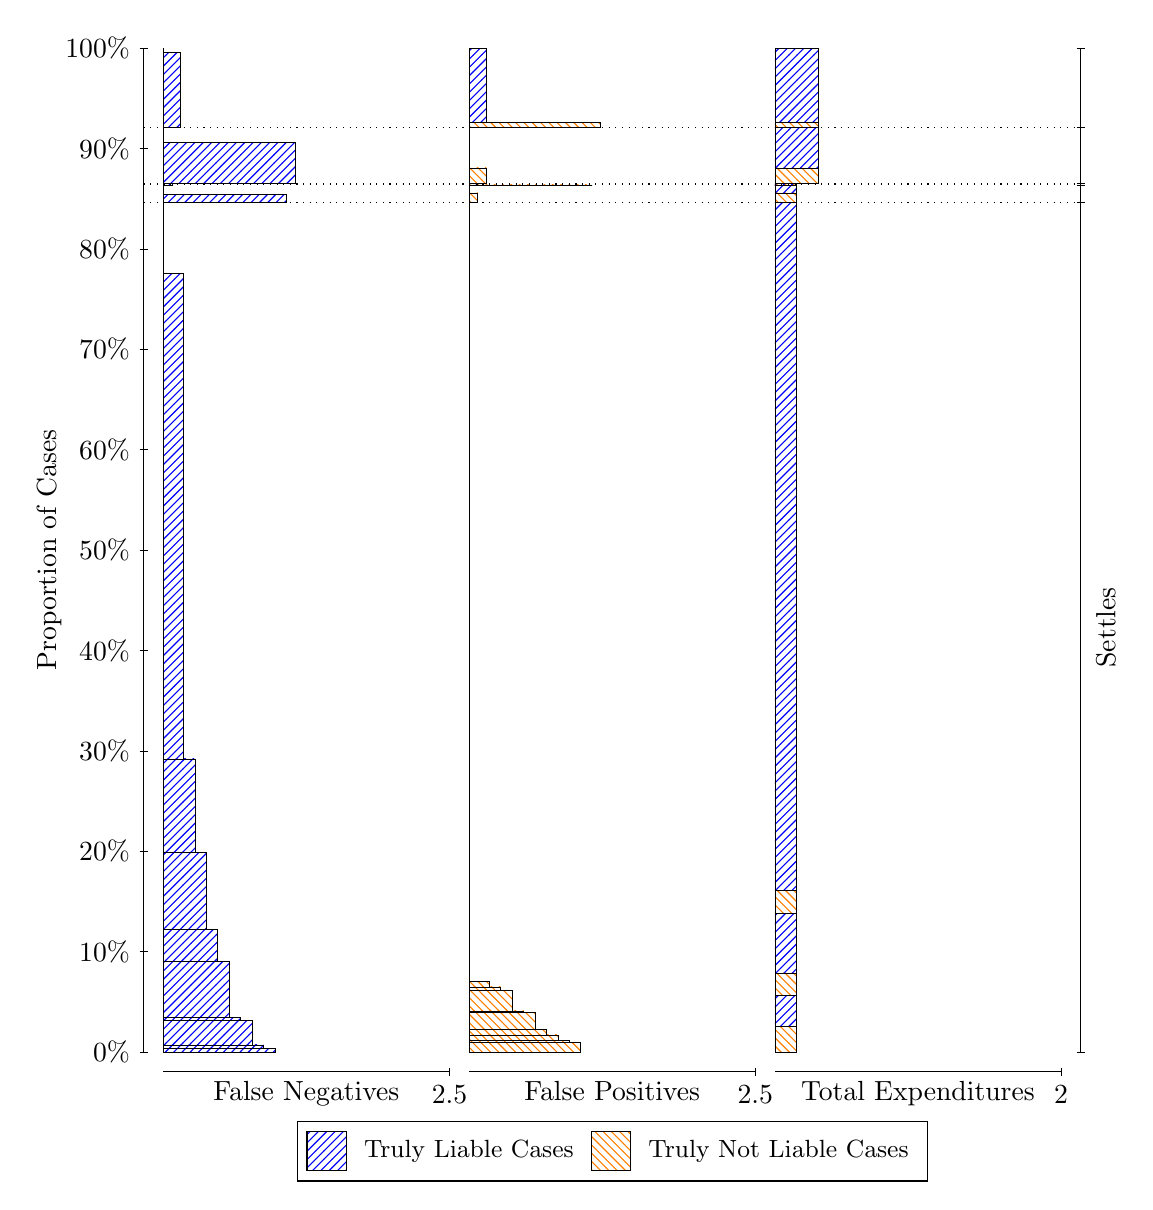
\begin{tikzpicture}
\draw[black, very thin] (1.5,1.75) -- (1.5,14.5);
\node[rotate=90, text=black, anchor=center] at (0.3, 8.125) {Proportion of Cases};
\draw[black, very thin] (1.45,1.75) -- (1.55,1.75);
\node[text=black, anchor=east] at (1.45, 1.75) {0\%};
\draw[black, very thin] (1.45,3.025) -- (1.55,3.025);
\node[text=black, anchor=east] at (1.45, 3.025) {10\%};
\draw[black, very thin] (1.45,4.3) -- (1.55,4.3);
\node[text=black, anchor=east] at (1.45, 4.3) {20\%};
\draw[black, very thin] (1.45,5.575) -- (1.55,5.575);
\node[text=black, anchor=east] at (1.45, 5.575) {30\%};
\draw[black, very thin] (1.45,6.85) -- (1.55,6.85);
\node[text=black, anchor=east] at (1.45, 6.85) {40\%};
\draw[black, very thin] (1.45,8.125) -- (1.55,8.125);
\node[text=black, anchor=east] at (1.45, 8.125) {50\%};
\draw[black, very thin] (1.45,9.4) -- (1.55,9.4);
\node[text=black, anchor=east] at (1.45, 9.4) {60\%};
\draw[black, very thin] (1.45,10.675) -- (1.55,10.675);
\node[text=black, anchor=east] at (1.45, 10.675) {70\%};
\draw[black, very thin] (1.45,11.95) -- (1.55,11.95);
\node[text=black, anchor=east] at (1.45, 11.95) {80\%};
\draw[black, very thin] (1.45,13.225) -- (1.55,13.225);
\node[text=black, anchor=east] at (1.45, 13.225) {90\%};
\draw[black, very thin] (1.45,14.5) -- (1.55,14.5);
\node[text=black, anchor=east] at (1.45, 14.5) {100\%};

\draw[black, very thin] (13.4,1.75) -- (13.4,14.5);
\draw[black, very thin] (13.35,1.75) -- (13.45,1.75);
\node[anchor=west] at (13.35, 1.75) {};
\draw[black, very thin] (13.35,12.536) -- (13.45,12.536);
\node[anchor=west] at (13.35, 12.536) {};
\draw[black, very thin] (13.35,12.762) -- (13.45,12.762);
\node[anchor=west] at (13.35, 12.762) {};
\draw[black, very thin] (13.35,12.784) -- (13.45,12.784);
\node[anchor=west] at (13.35, 12.784) {};
\draw[black, very thin] (13.35,13.494) -- (13.45,13.494);
\node[anchor=west] at (13.35, 13.494) {};
\draw[black, very thin] (13.35,14.5) -- (13.45,14.5);
\node[anchor=west] at (13.35, 14.5) {};

\draw[black, very thin, pattern color=blue, pattern=north east lines] (1.75,1.75) rectangle (3.167,1.7969);
\draw[black, very thin, pattern color=blue, pattern=north east lines] (1.75,1.7969) rectangle (3.0217,1.8399);
\draw[black, very thin, pattern color=blue, pattern=north east lines] (1.75,1.8399) rectangle (2.8763,2.1541);
\draw[black, very thin, pattern color=blue, pattern=north east lines] (1.75,2.1541) rectangle (2.731,2.1913);
\draw[black, very thin, pattern color=blue, pattern=north east lines] (1.75,2.1913) rectangle (2.5857,2.8994);
\draw[black, very thin, pattern color=blue, pattern=north east lines] (1.75,2.8994) rectangle (2.4403,3.3117);
\draw[black, very thin, pattern color=blue, pattern=north east lines] (1.75,3.3117) rectangle (2.295,4.2896);
\draw[black, very thin, pattern color=blue, pattern=north east lines] (1.75,4.2896) rectangle (2.1497,5.4726);
\draw[black, very thin, pattern color=blue, pattern=north east lines] (1.75,5.4726) rectangle (2.0043,11.637);
\draw[black, very thin, pattern color=orange, pattern=north west lines] (1.75,11.637) rectangle (1.75,12.536);
\draw[black, very thin, pattern color=blue, pattern=north east lines] (1.75,12.536) rectangle (3.3123,12.638);
\draw[black, very thin, pattern color=orange, pattern=north west lines] (1.75,12.638) rectangle (1.75,12.762);
\draw[black, very thin, pattern color=blue, pattern=north east lines] (1.75,12.762) rectangle (1.859,12.783);
\draw[black, very thin, pattern color=orange, pattern=north west lines] (1.75,12.783) rectangle (1.75,12.784);
\draw[black, very thin, pattern color=blue, pattern=north east lines] (1.75,12.784) rectangle (3.4213,13.299);
\draw[black, very thin, pattern color=orange, pattern=north west lines] (1.75,13.299) rectangle (1.75,13.494);
\draw[black, very thin, pattern color=blue, pattern=north east lines] (1.75,13.494) rectangle (1.968,14.443);
\draw[black, very thin, pattern color=orange, pattern=north west lines] (1.75,14.443) rectangle (1.75,14.5);
\draw[black, very thin, pattern color=orange, pattern=north west lines] (5.6333,1.75) rectangle (7.0503,1.8703);
\draw[black, very thin, pattern color=orange, pattern=north west lines] (5.6333,1.8703) rectangle (6.905,1.9001);
\draw[black, very thin, pattern color=orange, pattern=north west lines] (5.6333,1.9001) rectangle (6.7597,1.9658);
\draw[black, very thin, pattern color=orange, pattern=north west lines] (5.6333,1.9658) rectangle (6.6143,2.0397);
\draw[black, very thin, pattern color=orange, pattern=north west lines] (5.6333,2.0397) rectangle (6.469,2.2521);
\draw[black, very thin, pattern color=orange, pattern=north west lines] (5.6333,2.2521) rectangle (6.3237,2.2718);
\draw[black, very thin, pattern color=orange, pattern=north west lines] (5.6333,2.2718) rectangle (6.1783,2.5322);
\draw[black, very thin, pattern color=orange, pattern=north west lines] (5.6333,2.5322) rectangle (6.033,2.5764);
\draw[black, very thin, pattern color=orange, pattern=north west lines] (5.6333,2.5764) rectangle (5.8877,2.6492);
\draw[black, very thin, pattern color=blue, pattern=north east lines] (5.6333,2.6492) rectangle (5.6333,12.536);
\draw[black, very thin, pattern color=orange, pattern=north west lines] (5.6333,12.536) rectangle (5.7423,12.66);
\draw[black, very thin, pattern color=blue, pattern=north east lines] (5.6333,12.66) rectangle (5.6333,12.762);
\draw[black, very thin, pattern color=orange, pattern=north west lines] (5.6333,12.762) rectangle (7.1957,12.762);
\draw[black, very thin, pattern color=blue, pattern=north east lines] (5.6333,12.762) rectangle (5.7423,12.784);
\draw[black, very thin, pattern color=orange, pattern=north west lines] (5.6333,12.784) rectangle (5.8513,12.978);
\draw[black, very thin, pattern color=blue, pattern=north east lines] (5.6333,12.978) rectangle (5.6333,13.494);
\draw[black, very thin, pattern color=orange, pattern=north west lines] (5.6333,13.494) rectangle (7.3047,13.551);
\draw[black, very thin, pattern color=blue, pattern=north east lines] (5.6333,13.551) rectangle (5.8513,14.5);
\draw[black, very thin, pattern color=orange, pattern=north west lines] (9.5167,1.75) rectangle (9.7892,2.0743);
\draw[black, very thin, pattern color=blue, pattern=north east lines] (9.5167,2.0743) rectangle (9.7892,2.4687);
\draw[black, very thin, pattern color=orange, pattern=north west lines] (9.5167,2.4687) rectangle (9.7892,2.7539);
\draw[black, very thin, pattern color=blue, pattern=north east lines] (9.5167,2.7539) rectangle (9.7892,3.5089);
\draw[black, very thin, pattern color=orange, pattern=north west lines] (9.5167,3.5089) rectangle (9.7892,3.7986);
\draw[black, very thin, pattern color=blue, pattern=north east lines] (9.5167,3.7986) rectangle (9.7892,12.536);
\draw[black, very thin, pattern color=orange, pattern=north west lines] (9.5167,12.536) rectangle (9.7892,12.66);
\draw[black, very thin, pattern color=blue, pattern=north east lines] (9.5167,12.66) rectangle (9.7892,12.762);
\draw[black, very thin, pattern color=orange, pattern=north west lines] (9.5167,12.762) rectangle (9.7892,12.762);
\draw[black, very thin, pattern color=blue, pattern=north east lines] (9.5167,12.762) rectangle (9.7892,12.784);
\draw[black, very thin, pattern color=orange, pattern=north west lines] (9.5167,12.784) rectangle (10.062,12.978);
\draw[black, very thin, pattern color=blue, pattern=north east lines] (9.5167,12.978) rectangle (10.062,13.494);
\draw[black, very thin, pattern color=orange, pattern=north west lines] (9.5167,13.494) rectangle (10.062,13.551);
\draw[black, very thin, pattern color=blue, pattern=north east lines] (9.5167,13.551) rectangle (10.062,14.5);
\draw[black, dotted] (1.5,12.536) -- (13.4,12.536);
\draw[black, dotted] (1.5,12.762) -- (13.4,12.762);
\draw[black, dotted] (1.5,12.784) -- (13.4,12.784);
\draw[black, dotted] (1.5,13.494) -- (13.4,13.494);
\draw[black, very thin] (1.75,1.5) -- (5.3833,1.5);
\node[text=black, anchor=north] at (3.5667, 1.5) {False Negatives};
\draw[black, very thin] (5.3833,1.45) -- (5.3833,1.55);
\node[text=black, anchor=north] at (5.3833, 1.45) {2.5};

\draw[black, very thin] (5.6333,1.5) -- (9.2667,1.5);
\node[text=black, anchor=north] at (7.45, 1.5) {False Positives};
\draw[black, very thin] (9.2667,1.45) -- (9.2667,1.55);
\node[text=black, anchor=north] at (9.2667, 1.45) {2.5};

\draw[black, very thin] (9.5167,1.5) -- (13.15,1.5);
\node[text=black, anchor=north] at (11.333, 1.5) {Total Expenditures};
\draw[black, very thin] (13.15,1.45) -- (13.15,1.55);
\node[text=black, anchor=north] at (13.15, 1.45) {2};

\node[text=black, centered, rotate=90] at (13.72, 7.143) {Settles};





\draw (7.449999999999999,1.5) node[draw=none] (baseCoordinate) {};
\begin{scope}[align=center]
        \matrix[scale=0.5, draw=black, below=0.5cm of baseCoordinate, nodes={draw}, column sep=0.1cm]{
            \node[rectangle, draw, minimum width=0.5cm, minimum height=0.5cm, pattern color=blue, pattern=north east lines] {}; &
            \node[draw=none, font=\small, text=black] (B) {Truly Liable Cases}; &
            \node[rectangle, draw, minimum width=0.5cm, minimum height=0.5cm, pattern color=orange, pattern=north west lines] {}; &
            \node[draw=none, font=\small, text=black] (B) {Truly Not Liable Cases}; \\
            };
\end{scope}

\end{tikzpicture}
\end{document}